%!TeX root=../emmatop.tex
\chapter[Chapter \thechapter]{}
	
\lettrine[lraise=0.3]{N}{o} misfortune occurred, again to prevent the ball. The day approached, the day arrived; and after a morning of some anxious watching, Frank Churchill, in all the certainty of his own self, reached Randalls before dinner, and every thing was safe.

No second meeting had there yet been between him and Emma. The room at the Crown was to witness it;—but it would be better than a common meeting in a crowd. Mr Weston had been so very earnest in his entreaties for her arriving there as soon as possible after themselves, for the purpose of taking her opinion as to the propriety and comfort of the rooms before any other persons came, that she could not refuse him, and must therefore spend some quiet interval in the young man's company. She was to convey Harriet, and they drove to the Crown in good time, the Randalls party just sufficiently before them.

Frank Churchill seemed to have been on the watch; and though he did not say much, his eyes declared that he meant to have a delightful evening. They all walked about together, to see that every thing was as it should be; and within a few minutes were joined by the contents of another carriage, which Emma could not hear the sound of at first, without great surprize. <So unreasonably early!> she was going to exclaim; but she presently found that it was a family of old friends, who were coming, like herself, by particular desire, to help Mr Weston's judgment; and they were so very closely followed by another carriage of cousins, who had been entreated to come early with the same distinguishing earnestness, on the same errand, that it seemed as if half the company might soon be collected together for the purpose of preparatory inspection.

Emma perceived that her taste was not the only taste on which Mr Weston depended, and felt, that to be the favourite and intimate of a man who had so many intimates and confidantes, was not the very first distinction in the scale of vanity. She liked his open manners, but a little less of open-heartedness would have made him a higher character.—General benevolence, but not general friendship, made a man what he ought to be.—She could fancy such a man. The whole party walked about, and looked, and praised again; and then, having nothing else to do, formed a sort of half-circle round the fire, to observe in their various modes, till other subjects were started, that, though May, a fire in the evening was still very pleasant.

Emma found that it was not Mr Weston's fault that the number of privy councillors was not yet larger. They had stopped at Mrs Bates's door to offer the use of their carriage, but the aunt and niece were to be brought by the Eltons.

Frank was standing by her, but not steadily; there was a restlessness, which shewed a mind not at ease. He was looking about, he was going to the door, he was watching for the sound of other carriages,—impatient to begin, or afraid of being always near her.

Mrs Elton was spoken of. <I think she must be here soon,> said he. <I have a great curiosity to see Mrs Elton, I have heard so much of her. It cannot be long, I think, before she comes.>

A carriage was heard. He was on the move immediately; but coming back, said,

<I am forgetting that I am not acquainted with her. I have never seen either Mr or Mrs Elton. I have no business to put myself forward.>

Mr and Mrs Elton appeared; and all the smiles and the proprieties passed.

<But Miss Bates and Miss Fairfax!> said Mr Weston, looking about. <We thought you were to bring them.>

The mistake had been slight. The carriage was sent for them now. Emma longed to know what Frank's first opinion of Mrs Elton might be; how he was affected by the studied elegance of her dress, and her smiles of graciousness. He was immediately qualifying himself to form an opinion, by giving her very proper attention, after the introduction had passed.

In a few minutes the carriage returned.—Somebody talked of rain.—<I will see that there are umbrellas, sir,> said Frank to his father: <Miss Bates must not be forgotten:> and away he went. Mr Weston was following; but Mrs Elton detained him, to gratify him by her opinion of his son; and so briskly did she begin, that the young man himself, though by no means moving slowly, could hardly be out of hearing.

<A very fine young man indeed, Mr Weston. You know I candidly told you I should form my own opinion; and I am happy to say that I am extremely pleased with him.—You may believe me. I never compliment. I think him a very handsome young man, and his manners are precisely what I like and approve—so truly the gentleman, without the least conceit or puppyism. You must know I have a vast dislike to puppies—quite a horror of them. They were never tolerated at Maple Grove. Neither Mr Suckling nor me had ever any patience with them; and we used sometimes to say very cutting things! Selina, who is mild almost to a fault, bore with them much better.>

While she talked of his son, Mr Weston's attention was chained; but when she got to Maple Grove, he could recollect that there were ladies just arriving to be attended to, and with happy smiles must hurry away.

Mrs Elton turned to Mrs Weston. <I have no doubt of its being our carriage with Miss Bates and Jane. Our coachman and horses are so extremely expeditious!—I believe we drive faster than any body.—What a pleasure it is to send one's carriage for a friend!—I understand you were so kind as to offer, but another time it will be quite unnecessary. You may be very sure I shall always take care of them.>

Miss Bates and Miss Fairfax, escorted by the two gentlemen, walked into the room; and Mrs Elton seemed to think it as much her duty as Mrs Weston's to receive them. Her gestures and movements might be understood by any one who looked on like Emma; but her words, every body's words, were soon lost under the incessant flow of Miss Bates, who came in talking, and had not finished her speech under many minutes after her being admitted into the circle at the fire. As the door opened she was heard,

\begin{figure}[tbph]
\centering
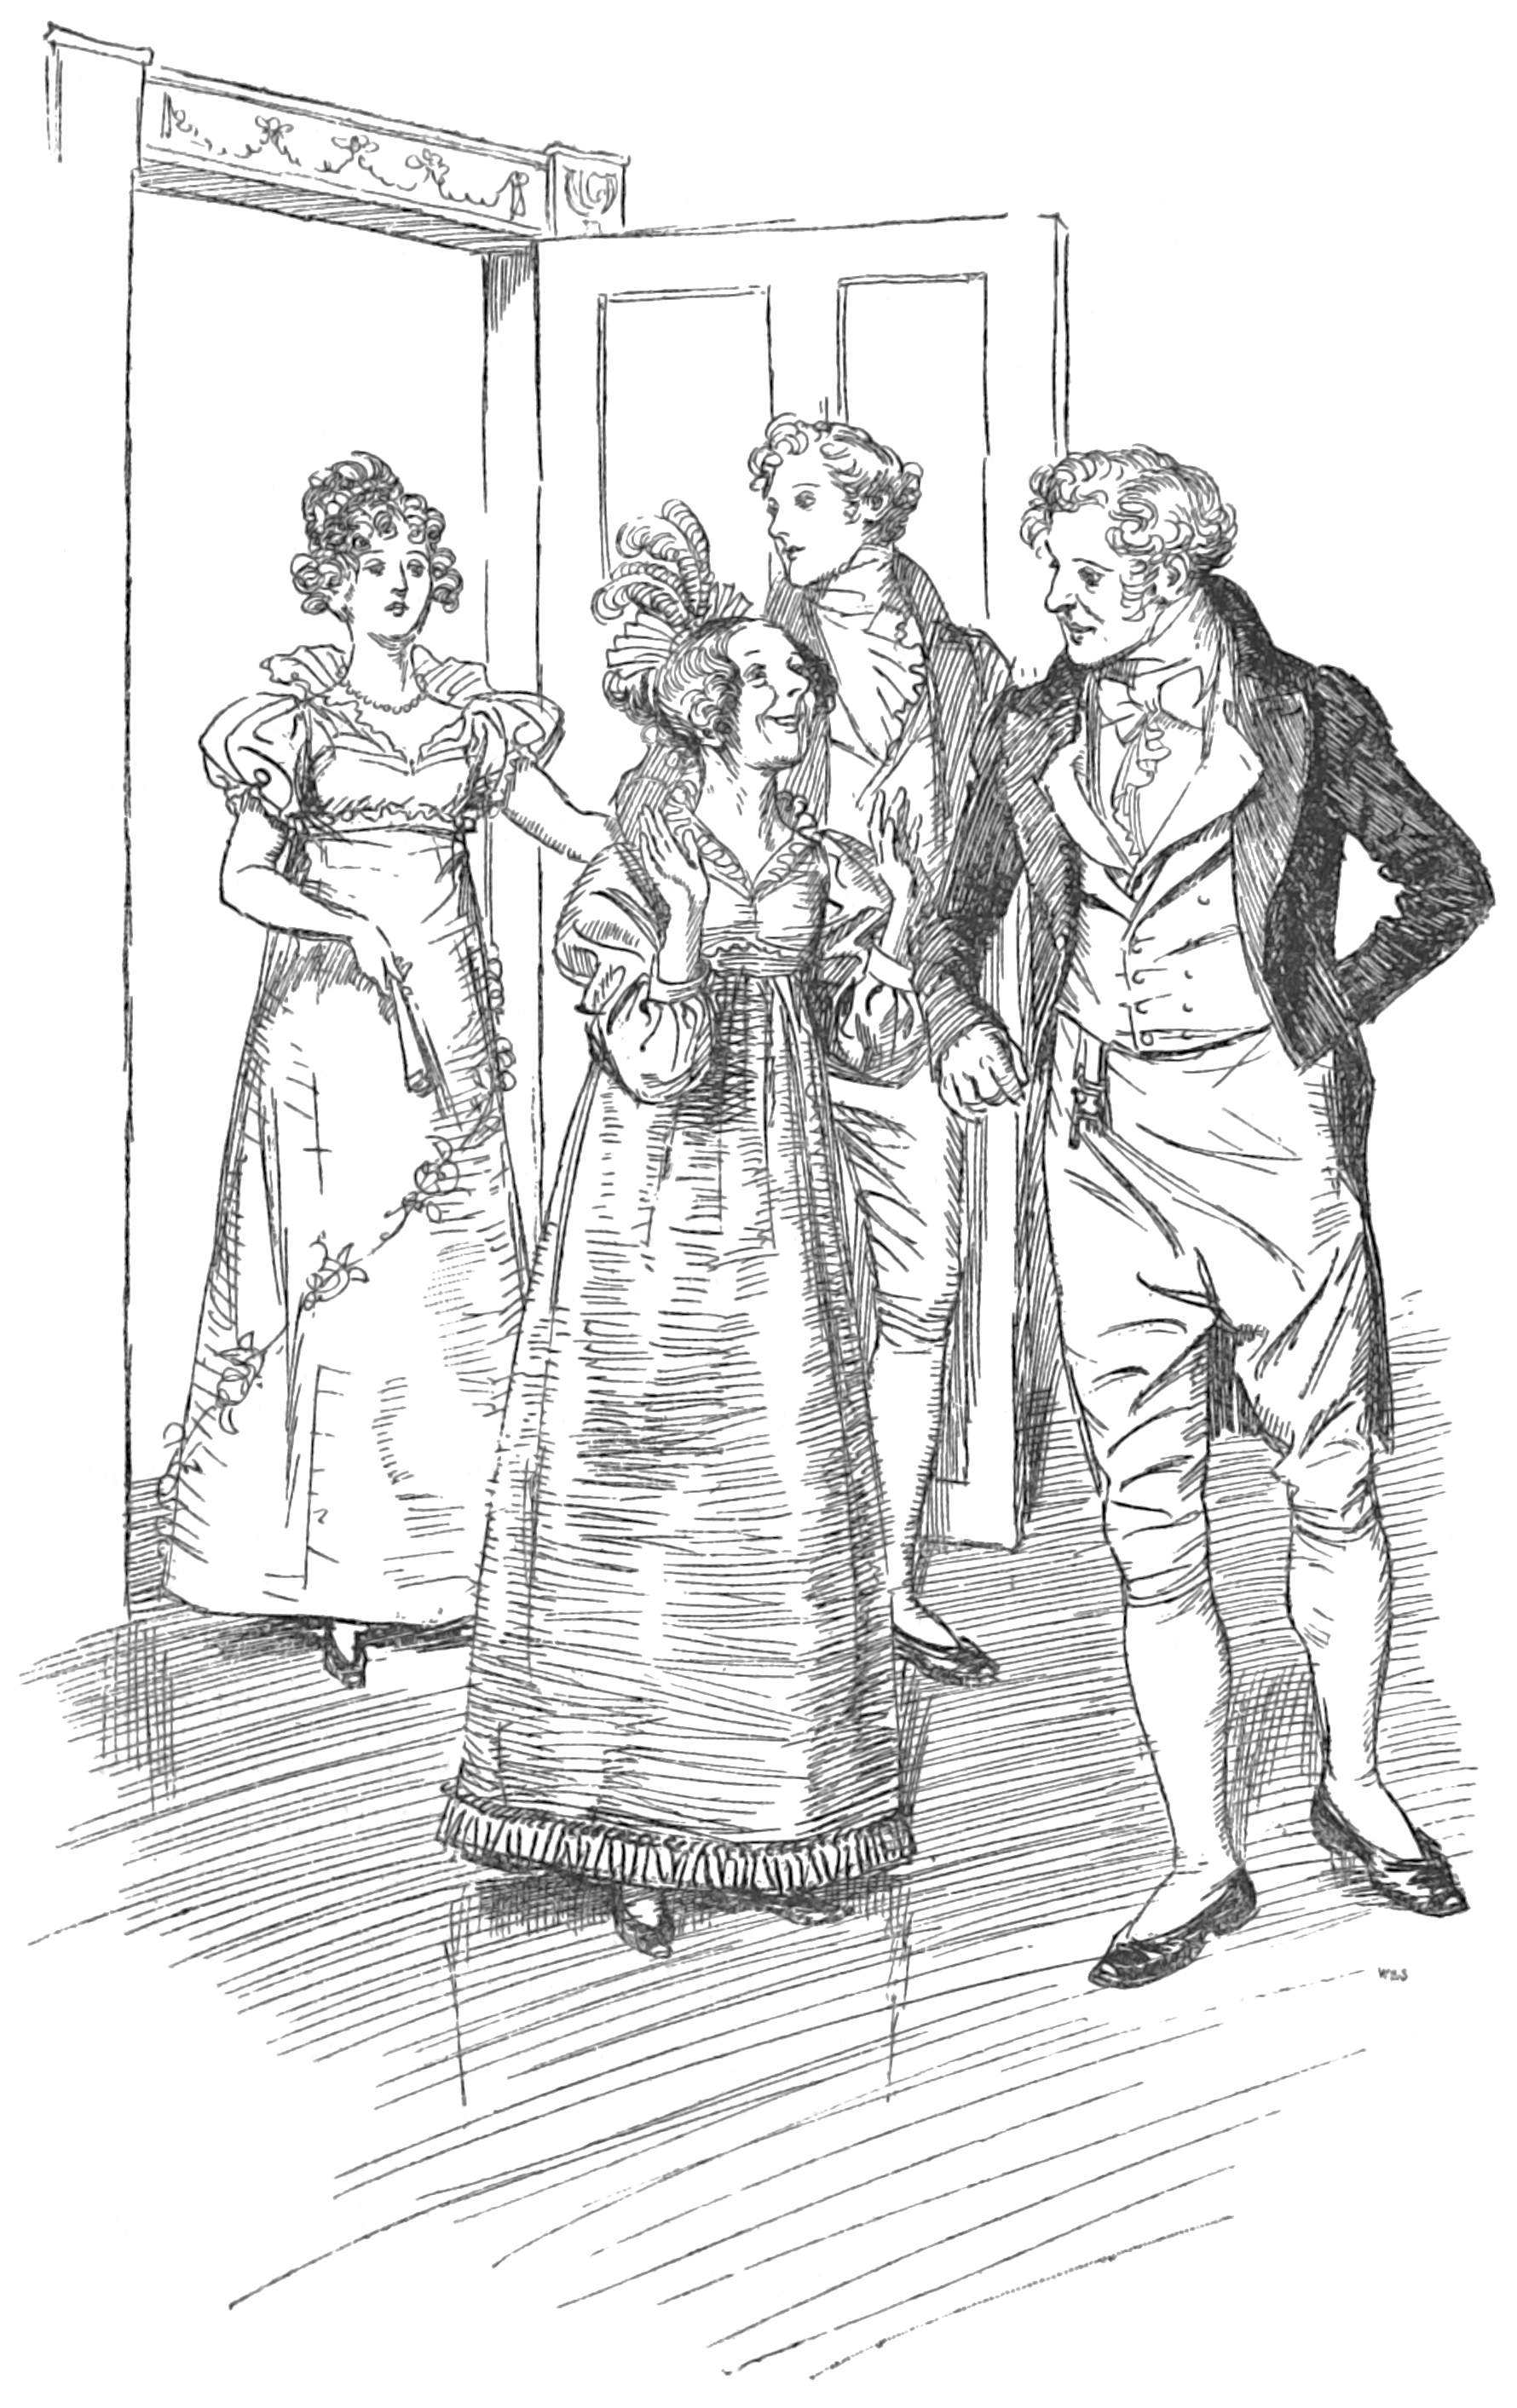
\includegraphics[width=.9\linewidth]{38brilliant}
\caption{<Oh! This is brilliant, indeed!>}
\end{figure}

<So very obliging of you!—No rain at all. Nothing to signify. I do not care for myself. Quite thick shoes. And Jane declares—Well!—(as soon as she was within the door) Well! This is brilliant indeed!—This is admirable!—Excellently contrived, upon my word. Nothing wanting. Could not have imagined it.—So well lighted up!—Jane, Jane, look!—did you ever see any thing? Oh! Mr Weston, you must really have had Aladdin's lamp. Good Mrs Stokes would not know her own room again. I saw her as I came in; she was standing in the entrance. <Oh! Mrs Stokes,> said I—but I had not time for more.> She was now met by Mrs Weston.—<Very well, I thank you, ma'am. I hope you are quite well. Very happy to hear it. So afraid you might have a headache!—seeing you pass by so often, and knowing how much trouble you must have. Delighted to hear it indeed. Ah! dear Mrs Elton, so obliged to you for the carriage!—excellent time. Jane and I quite ready. Did not keep the horses a moment. Most comfortable carriage.—Oh! and I am sure our thanks are due to you, Mrs Weston, on that score. Mrs Elton had most kindly sent Jane a note, or we should have been.—But two such offers in one day!—Never were such neighbours. I said to my mother, <Upon my word, ma'am—.> Thank you, my mother is remarkably well. Gone to Mr Woodhouse's. I made her take her shawl—for the evenings are not warm—her large new shawl— Mrs Dixon's wedding-present.—So kind of her to think of my mother! Bought at Weymouth, you know—Mr Dixon's choice. There were three others, Jane says, which they hesitated about some time. Colonel Campbell rather preferred an olive. My dear Jane, are you sure you did not wet your feet?—It was but a drop or two, but I am so afraid:—but Mr Frank Churchill was so extremely—and there was a mat to step upon—I shall never forget his extreme politeness.—Oh! Mr Frank Churchill, I must tell you my mother's spectacles have never been in fault since; the rivet never came out again. My mother often talks of your good-nature. Does not she, Jane?—Do not we often talk of Mr Frank Churchill?—Ah! here's Miss Woodhouse.—Dear Miss Woodhouse, how do you do?—Very well I thank you, quite well. This is meeting quite in fairy-land!—Such a transformation!—Must not compliment, I know (eyeing Emma most complacently)—that would be rude—but upon my word, Miss Woodhouse, you do look—how do you like Jane's hair?—You are a judge.—She did it all herself. Quite wonderful how she does her hair!—No hairdresser from London I think could.—Ah! Dr Hughes I declare—and Mrs Hughes. Must go and speak to Dr and Mrs Hughes for a moment.—How do you do? How do you do?—Very well, I thank you. This is delightful, is not it?—Where's dear Mr Richard?—Oh! there he is. Don't disturb him. Much better employed talking to the young ladies. How do you do, Mr Richard?—I saw you the other day as you rode through the town—Mrs Otway, I protest!—and good Mr Otway, and Miss Otway and Miss Caroline.—Such a host of friends!—and Mr George and Mr Arthur!—How do you do? How do you all do?—Quite well, I am much obliged to you. Never better.—Don't I hear another carriage?—Who can this be?—very likely the worthy Coles.—Upon my word, this is charming to be standing about among such friends! And such a noble fire!—I am quite roasted. No coffee, I thank you, for me—never take coffee.—A little tea if you please, sir, by and bye,—no hurry—Oh! here it comes. Every thing so good!>

Frank Churchill returned to his station by Emma; and as soon as Miss Bates was quiet, she found herself necessarily overhearing the discourse of Mrs Elton and Miss Fairfax, who were standing a little way behind her.—He was thoughtful. Whether he were overhearing too, she could not determine. After a good many compliments to Jane on her dress and look, compliments very quietly and properly taken, Mrs Elton was evidently wanting to be complimented herself—and it was, <How do you like my gown?—How do you like my trimming?—How has Wright done my hair?>—with many other relative questions, all answered with patient politeness. Mrs Elton then said, <Nobody can think less of dress in general than I do—but upon such an occasion as this, when every body's eyes are so much upon me, and in compliment to the Westons—who I have no doubt are giving this ball chiefly to do me honour—I would not wish to be inferior to others. And I see very few pearls in the room except mine.—So Frank Churchill is a capital dancer, I understand.—We shall see if our styles suit.—A fine young man certainly is Frank Churchill. I like him very well.>



At this moment Frank began talking so vigorously, that Emma could not but imagine he had overheard his own praises, and did not want to hear more;—and the voices of the ladies were drowned for a while, till another suspension brought Mrs Elton's tones again distinctly forward.—Mr Elton had just joined them, and his wife was exclaiming,

<Oh! you have found us out at last, have you, in our seclusion?—I was this moment telling Jane, I thought you would begin to be impatient for tidings of us.>

<Jane!>—repeated Frank Churchill, with a look of surprize and displeasure.—<That is easy—but Miss Fairfax does not disapprove it, I suppose.>

<How do you like Mrs Elton?> said Emma in a whisper.

<Not at all.>

<You are ungrateful.>

<Ungrateful!—What do you mean?> Then changing from a frown to a smile—<No, do not tell me—I do not want to know what you mean.—Where is my father?—When are we to begin dancing?>

Emma could hardly understand him; he seemed in an odd humour. He walked off to find his father, but was quickly back again with both Mr and Mrs Weston. He had met with them in a little perplexity, which must be laid before Emma. It had just occurred to Mrs Weston that Mrs Elton must be asked to begin the ball; that she would expect it; which interfered with all their wishes of giving Emma that distinction.—Emma heard the sad truth with fortitude.

<And what are we to do for a proper partner for her?> said Mr Weston. <She will think Frank ought to ask her.>

\begin{figure}[tbph]
\centering
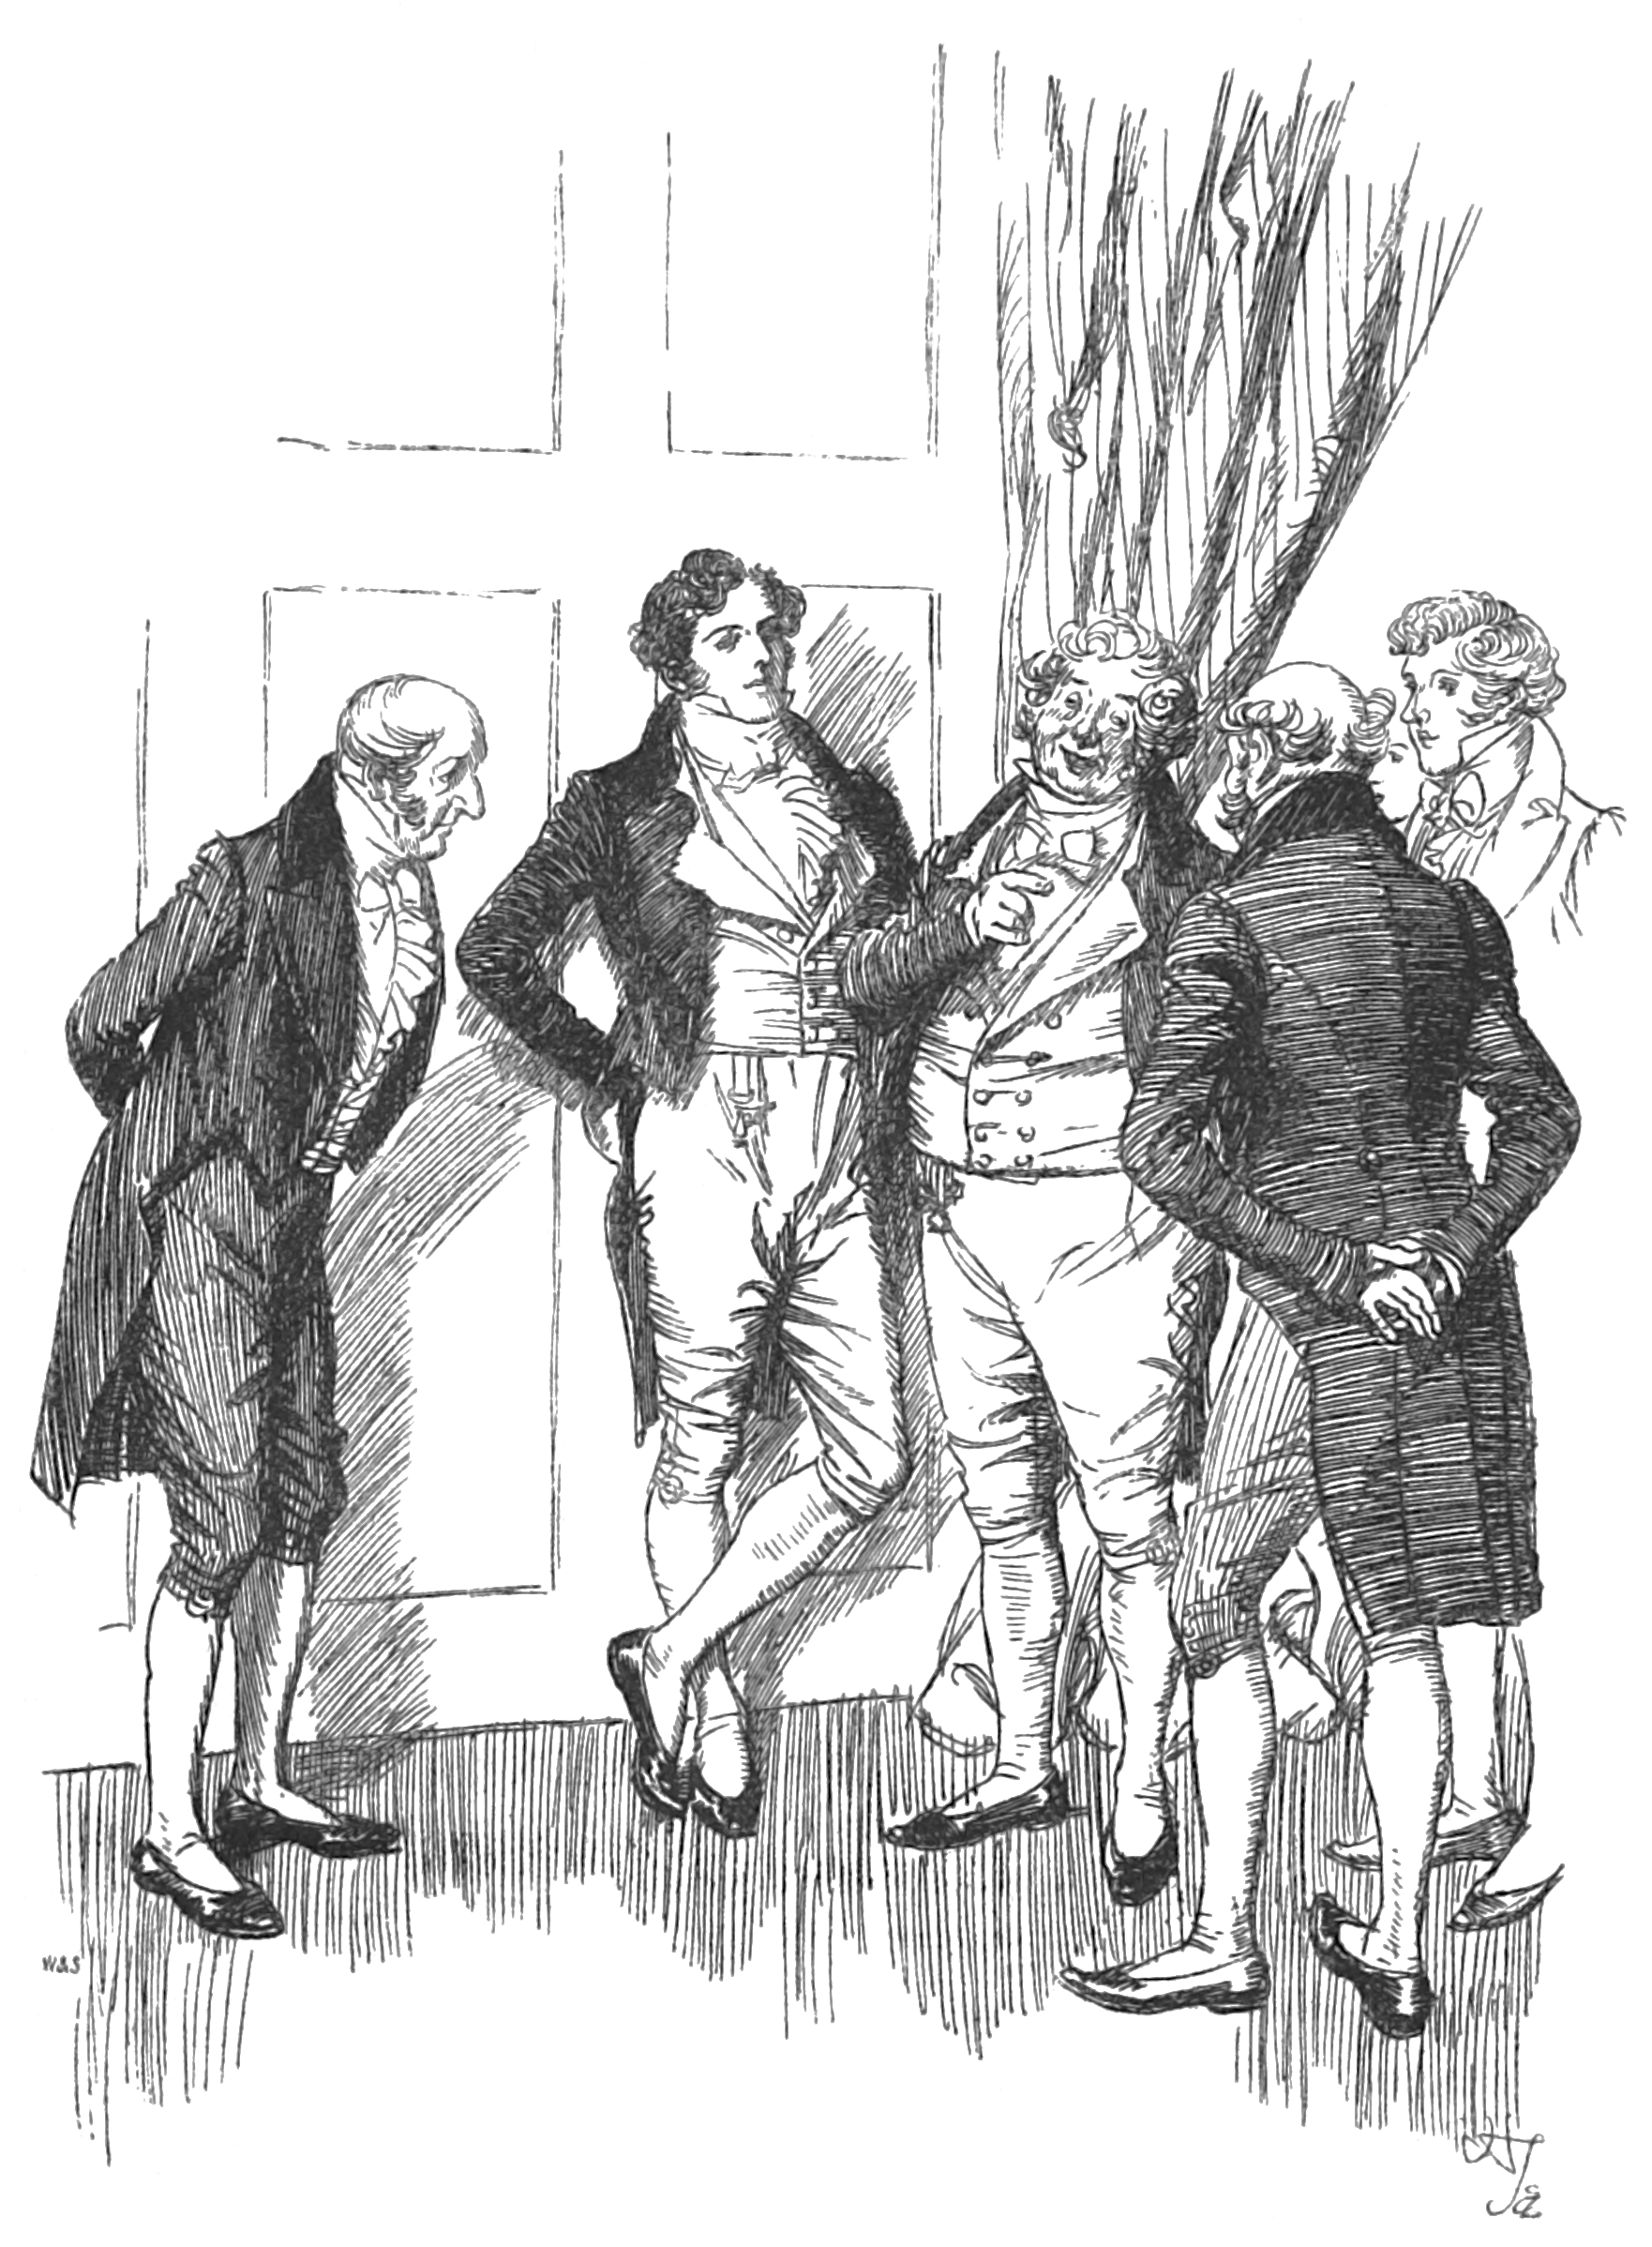
\includegraphics[width=.9\linewidth]{38bulky}
\caption{Among the bulky forms and stooping shoulders}
\end{figure}

Frank turned instantly to Emma, to claim her former promise; and boasted himself an engaged man, which his father looked his most perfect approbation of—and it then appeared that Mrs Weston was wanting him to dance with Mrs Elton himself, and that their business was to help to persuade him into it, which was done pretty soon.—Mr Weston and Mrs Elton led the way, Mr Frank Churchill and Miss Woodhouse followed. Emma must submit to stand second to Mrs Elton, though she had always considered the ball as peculiarly for her. It was almost enough to make her think of marrying. Mrs Elton had undoubtedly the advantage, at this time, in vanity completely gratified; for though she had intended to begin with Frank Churchill, she could not lose by the change. Mr Weston might be his son's superior.—In spite of this little rub, however, Emma was smiling with enjoyment, delighted to see the respectable length of the set as it was forming, and to feel that she had so many hours of unusual festivity before her.—She was more disturbed by Mr Knightley's not dancing than by any thing else.—There he was, among the standers-by, where he ought not to be; he ought to be dancing,—not classing himself with the husbands, and fathers, and whist-players, who were pretending to feel an interest in the dance till their rubbers were made up,—so young as he looked!—He could not have appeared to greater advantage perhaps anywhere, than where he had placed himself. His tall, firm, upright figure, among the bulky forms and stooping shoulders of the elderly men, was such as Emma felt must draw every body's eyes; and, excepting her own partner, there was not one among the whole row of young men who could be compared with him.—He moved a few steps nearer, and those few steps were enough to prove in how gentlemanlike a manner, with what natural grace, he must have danced, would he but take the trouble.—Whenever she caught his eye, she forced him to smile; but in general he was looking grave. She wished he could love a ballroom better, and could like Frank Churchill better.—He seemed often observing her. She must not flatter herself that he thought of her dancing, but if he were criticising her behaviour, she did not feel afraid. There was nothing like flirtation between her and her partner. They seemed more like cheerful, easy friends, than lovers. That Frank Churchill thought less of her than he had done, was indubitable.

The ball proceeded pleasantly. The anxious cares, the incessant attentions of Mrs Weston, were not thrown away. Every body seemed happy; and the praise of being a delightful ball, which is seldom bestowed till after a ball has ceased to be, was repeatedly given in the very beginning of the existence of this. Of very important, very recordable events, it was not more productive than such meetings usually are. There was one, however, which Emma thought something of.—The two last dances before supper were begun, and Harriet had no partner;—the only young lady sitting down;—and so equal had been hitherto the number of dancers, that how there could be any one disengaged was the wonder!—But Emma's wonder lessened soon afterwards, on seeing Mr Elton sauntering about. He would not ask Harriet to dance if it were possible to be avoided: she was sure he would not—and she was expecting him every moment to escape into the card-room.

Escape, however, was not his plan. He came to the part of the room where the sitters-by were collected, spoke to some, and walked about in front of them, as if to shew his liberty, and his resolution of maintaining it. He did not omit being sometimes directly before Miss Smith, or speaking to those who were close to her.—Emma saw it. She was not yet dancing; she was working her way up from the bottom, and had therefore leisure to look around, and by only turning her head a little she saw it all. When she was half-way up the set, the whole group were exactly behind her, and she would no longer allow her eyes to watch; but Mr Elton was so near, that she heard every syllable of a dialogue which just then took place between him and Mrs Weston; and she perceived that his wife, who was standing immediately above her, was not only listening also, but even encouraging him by significant glances.—The kind-hearted, gentle Mrs Weston had left her seat to join him and say, <Do not you dance, Mr Elton?> to which his prompt reply was, <Most readily, Mrs Weston, if you will dance with me.>

<Me!—oh! no—I would get you a better partner than myself. I am no dancer.>

<If Mrs Gilbert wishes to dance,> said he, <I shall have great pleasure, I am sure—for, though beginning to feel myself rather an old married man, and that my dancing days are over, it would give me very great pleasure at any time to stand up with an old friend like Mrs Gilbert.>

<Mrs Gilbert does not mean to dance, but there is a young lady disengaged whom I should be very glad to see dancing—Miss Smith.> <Miss Smith!—oh!—I had not observed.—You are extremely obliging—and if I were not an old married man.—But my dancing days are over, Mrs Weston. You will excuse me. Any thing else I should be most happy to do, at your command—but my dancing days are over.>

Mrs Weston said no more; and Emma could imagine with what surprize and mortification she must be returning to her seat. This was Mr Elton! the amiable, obliging, gentle Mr Elton.—She looked round for a moment; he had joined Mr Knightley at a little distance, and was arranging himself for settled conversation, while smiles of high glee passed between him and his wife.

She would not look again. Her heart was in a glow, and she feared her face might be as hot.

In another moment a happier sight caught her;—Mr Knightley leading Harriet to the set!—Never had she been more surprized, seldom more delighted, than at that instant. She was all pleasure and gratitude, both for Harriet and herself, and longed to be thanking him; and though too distant for speech, her countenance said much, as soon as she could catch his eye again.

His dancing proved to be just what she had believed it, extremely good; and Harriet would have seemed almost too lucky, if it had not been for the cruel state of things before, and for the very complete enjoyment and very high sense of the distinction which her happy features announced. It was not thrown away on her, she bounded higher than ever, flew farther down the middle, and was in a continual course of smiles.

Mr Elton had retreated into the card-room, looking (Emma trusted) very foolish. She did not think he was quite so hardened as his wife, though growing very like her;—she spoke some of her feelings, by observing audibly to her partner,

<Knightley has taken pity on poor little Miss Smith!—Very good-natured, I declare.>

Supper was announced. The move began; and Miss Bates might be heard from that moment, without interruption, till her being seated at table and taking up her spoon.

<Jane, Jane, my dear Jane, where are you?—Here is your tippet. Mrs Weston begs you to put on your tippet. She says she is afraid there will be draughts in the passage, though every thing has been done—One door nailed up—Quantities of matting—My dear Jane, indeed you must. Mr Churchill, oh! you are too obliging! How well you put it on!—so gratified! Excellent dancing indeed!—Yes, my dear, I ran home, as I said I should, to help grandmama to bed, and got back again, and nobody missed me.—I set off without saying a word, just as I told you. Grandmama was quite well, had a charming evening with Mr Woodhouse, a vast deal of chat, and backgammon.—Tea was made downstairs, biscuits and baked apples and wine before she came away: amazing luck in some of her throws: and she inquired a great deal about you, how you were amused, and who were your partners. <Oh!> said I, <I shall not forestall Jane; I left her dancing with Mr George Otway; she will love to tell you all about it herself to-morrow: her first partner was Mr Elton, I do not know who will ask her next, perhaps Mr William Cox.> My dear sir, you are too obliging.—Is there nobody you would not rather?—I am not helpless. Sir, you are most kind. Upon my word, Jane on one arm, and me on the other!—Stop, stop, let us stand a little back, Mrs Elton is going; dear Mrs Elton, how elegant she looks!—Beautiful lace!—Now we all follow in her train. Quite the queen of the evening!—Well, here we are at the passage. Two steps, Jane, take care of the two steps. Oh! no, there is but one. Well, I was persuaded there were two. How very odd! I was convinced there were two, and there is but one. I never saw any thing equal to the comfort and style—Candles everywhere.—I was telling you of your grandmama, Jane,—There was a little disappointment.—The baked apples and biscuits, excellent in their way, you know; but there was a delicate fricassee of sweetbread and some asparagus brought in at first, and good Mr Woodhouse, not thinking the asparagus quite boiled enough, sent it all out again. Now there is nothing grandmama loves better than sweetbread and asparagus—so she was rather disappointed, but we agreed we would not speak of it to any body, for fear of its getting round to dear Miss Woodhouse, who would be so very much concerned!—Well, this is brilliant! I am all amazement! could not have supposed any thing!—Such elegance and profusion!—I have seen nothing like it since—Well, where shall we sit? where shall we sit? Anywhere, so that Jane is not in a draught. Where I sit is of no consequence. Oh! do you recommend this side?—Well, I am sure, Mr Churchill—only it seems too good—but just as you please. What you direct in this house cannot be wrong. Dear Jane, how shall we ever recollect half the dishes for grandmama? Soup too! Bless me! I should not be helped so soon, but it smells most excellent, and I cannot help beginning.>

Emma had no opportunity of speaking to Mr Knightley till after supper; but, when they were all in the ballroom again, her eyes invited him irresistibly to come to her and be thanked. He was warm in his reprobation of Mr Elton's conduct; it had been unpardonable rudeness; and Mrs Elton's looks also received the due share of censure.

<They aimed at wounding more than Harriet,> said he. <Emma, why is it that they are your enemies?>

He looked with smiling penetration; and, on receiving no answer, added, <She ought not to be angry with you, I suspect, whatever he may be.—To that surmise, you say nothing, of course; but confess, Emma, that you did want him to marry Harriet.>

<I did,> replied Emma, <and they cannot forgive me.>

He shook his head; but there was a smile of indulgence with it, and he only said,

<I shall not scold you. I leave you to your own reflections.>

<Can you trust me with such flatterers?—Does my vain spirit ever tell me I am wrong?>

<Not your vain spirit, but your serious spirit.—If one leads you wrong, I am sure the other tells you of it.>

<I do own myself to have been completely mistaken in Mr Elton. There is a littleness about him which you discovered, and which I did not: and I was fully convinced of his being in love with Harriet. It was through a series of strange blunders!>

<And, in return for your acknowledging so much, I will do you the justice to say, that you would have chosen for him better than he has chosen for himself.—Harriet Smith has some first-rate qualities, which Mrs Elton is totally without. An unpretending, single-minded, artless girl—infinitely to be preferred by any man of sense and taste to such a woman as Mrs Elton. I found Harriet more conversable than I expected.>

Emma was extremely gratified.—They were interrupted by the bustle of Mr Weston calling on every body to begin dancing again.

<Come Miss Woodhouse, Miss Otway, Miss Fairfax, what are you all doing?—Come Emma, set your companions the example. Every body is lazy! Every body is asleep!>

<I am ready,> said Emma, <whenever I am wanted.>

<Whom are you going to dance with?> asked Mr Knightley.

She hesitated a moment, and then replied, <With you, if you will ask me.>

<Will you?> said he, offering his hand.

<Indeed I will. You have shewn that you can dance, and you know we are not really so much brother and sister as to make it at all improper.>

<Brother and sister! no, indeed.>